
\section{Software Implementation}
The following subsections detail the implementation of the final software solution that has been written to meet the objectives posed at the beginning of this dissertation.

\subsection{Third Party FE Application}
In order to demonstrate the potential feasibility of the hybrid approach it was first important to obtain a finite element solver which could be given a FE model containing data about forces, materials and the mesh structure and then execute the model pro grammatically so as to obtain stress results. \\ 

\noindent
A multitude of commercial FE tools exist with there being a wide variety in both the complexity and cost associated with each tool. 
Finite element software is typically very expensive due to its high development cost and small customer base. Tools used within industry such as ANSYS typically require a great deal of time in order to become proficient in their usage and can cost in excess of five thousand pounds a year for a single licence \cite{AnsysCost}. It was therefore important to find a tool which was both affordable while also powerful enough to demonstrate a working prototype of the re meshing method.
 
\subsection{LISA}
After reviewing several FE applications used within industry in addition to a variety of less well known ones used within academia and by hobbyists LISA  was selected as the solver application for which to implement  the systems prototypes. \\ 

\noindent
\textbf{Strengths: }LISA as a FE tool which allows the user to run models of up to 1300 element for free; This was beneficial in allowing me to experiment with the software and gauge the feasibility of my projects concept before requiring a full version. Once at a stage in the project where each problem had been solved for small models containing less than 1300 elements an academic licence for the software was purchased for the projects use. \\

\noindent
LISA also provides a GUI which allows visual inspection of the model and its mesh; This is particularly useful for observing the output of the meshing algorithms which can often provide a human with a much better understanding of how the method has performed and whether or not there are obvious bugs. in the implementation of the meshing procedures \\ 

\noindent
\textbf{Weaknesses: } Due to LISA’s simplicity it does not come with an extensive API allowing for easy programmatic use of its inbuilt features, however it is still possible to interface with LISA through less direct means \cite{LISAManual}. LISA models are stored in .liml files which use XML as a meta mark-up format. The model files contain all the information about the model including the materials used as well as loads and constraints and of course the mesh. It is therefore possible to manipulate a .liml file having parsed its contents before writing a new version of the file which LISA can be called to solve. In order to more easily alter the model it made sense to write a wrapper  for the .liml files to abstract the manipulation of their content.

\subsection{Languages and platforms}
The final system has been written entirely using the C\# programming language (version 5.0) with Visual Studio 2015 as the development environment on a Windows 10 system. C\# is an application development language built on the .NET framework. Although any number of programming languages could have been used to implement the solution C\# offered a good compromise for developing a system with both structural rigidity through static typing and object orientation in addition to functionality to allow for rapid prototyping. C\# does this well through use of LINQ, a part of the standard library that provides a large number of higher order functions which allow for operations to be performed over any data structure that implements the built in IEnumerable interface. Given that much of the code within the project performs the same operation on collections of nodes and elements stored in Lists arrays and dictionaries which all implement IEnumerable the ability to write much of the project using this capability dramatically reduced the number of errors encountered and increased development speed.


\subsection{Implementation Methodology}
Growing size of the software meant it was important to work systematically to continuously drive the project in the right direction and avoid the introduction of unnecessary complexity. This was achieved through regularly reviewing and refactoring the code which dramatically helped to reduced the amount of bugs introduced. \\

\noindent
For the duration of the project the spiral methodology was adhered to. This enforced multiple deliverable stages that were concluded with a supervisor meeting every one or two weeks. Adopting the spiral methodology also provided flexibility regarding the order in which tasks were able to take place outside of a spiral iteration. This was necessary when conducing a research driven project where direction of work for subsequent development iterations was largely driven by the  findings of the work in the previous ones. \\

\noindent
Tasks were chosen every week for the project, the number of tasks and their complexity was determined using a combination of factors including their complexity, the criticality of the task e.g. Did it need to be completed for other important tasks to be started and the time available to me as the individual undertaking the project (More tasks typically performed on weeks when less work was due for other modules.

\subsection{Implementation of Subsystems}
This section describes the implementation details of the various different subsystems which combine to form the overall solution.

\subsubsection{Re-meshing using hierarchical refinement}
After reviewing both h-refinement \cite{HandPRefinements} and r-refinement \cite{RRefinement} it was concluded h-refinement would be best the best approach to adopt due to its simplicity and more widespread use \cite{HandPRefinements} despite the fact that the mesh is usually more computationally expensive than it would have been if it was created using r-refinement \cite{RRefinement}\\ 

\noindent
Elements within traditional FEA can typically be classified as either triangle or square based elements, each of these provide different strengths and weaknesses when required to mesh and solve models. Within industry triangular elements are typically preferable since it is always possible to generate an initial triangular mesh from any arbitrary CAD geometry algorithmically. This is done by simply making smaller triangles until all gaps along the edge of the geometry are filled \cite{DelaunyTriangles}. The same cannot always be said  when meshing using square elements. For proof of the solutions concept however it was concluded that square based elements were preferable to triangular ones with since the steps required for a basic refinement are much simpler, just take the corners of an element that already exists, add their x, y and z components before dividing each component by two to achieve the coordinate for a node which is halfway between the two. \\ 

\noindent
In addition to refinement it is also significantly easier to define edges which the ILP rules can be applied to when edges naturally form within a structure through a chain of nodes along the edges of square elements.

%The process of re meshing square based elements 

\noindent
Unfortunately Triangular meshes also generally incur a higher computational cost than an equivalent square element mesh due to added complexity of performing the calculations required to remesh in addition to requiring more elements over a given area to achieve the same accuracy. \\

\noindent
From an implementation standpoint writing a square based remeshing algorithm is also substantially easier as given an initial mesh made just of square elements the only task is to repeatedly divide each element into four sub elements, by contrast methods uses to re mesh triangular meshes vary greatly are typically more complex and have corresponding initial meshes that are harder to generate manually by human operators \cite{HandMeshing}. \\ 

\subsection{Fast node lookup and update of nodes}
A key requirement for the design of the data model generated by the hierarchical re meshing process was the need to perform fast lookup of nodes already present in the mesh. Lookup is important within the meshing methods as a means of checking whether a node that is about to be created already exists within the model, in the event that no such node already exists a new one can be created however if it does then instead of creating a new node the node that already exists needs to be connected to a node in an adjacent element that is currently being refined. If nodes are not linked correctly form correct elements the physics solver is unable to assume the stress moves through one element to another despite both having nodes at the same coordinates, this results in inaccurate output or potentially an error being thrown by LISA. \\ 

\noindent
This issue arose as a result of partly as a result of the systems design, as previously mentioned subdivision for every individual element is the responsibility of that element which from a software engineering perspective is very good since it means the low level meshing process for each different type of element could be written within that elements class. This avoids the need for much heavier generalised refinement classes that would have needed to know how to perform the meshing for all elements in the model at once and for each of the different potential element types. A consequence of this was despite every Element being capable of meshing itself perfectly adjacent elements that also requiring refinement needed the ability to reconnect the new nodes along their edges to those that had created by the adjacent element. \colorbox{yellow}{This can be seen below in figure x} \\ 


\begin{figure}[!h]
  \centerline{\includegraphics[width=100mm , scale=1]{../Graphics/nodeLinking.png}}
  \caption{The need for an element to check for existing adjacent nodes when subdividing itself during refinement,\\ \\
  	Orange Nodes - An original node for one or more elements \\
	Red Nodes - new nodes made by Elem A \\
	Purple Nodes - new nodes made by Elem B \\
  }
  \label{fig:h-refinementImp}
\end{figure}


\noindent
The solution to this problem was to store all the nodes in the mesh model within a C\# dictionary structure a reference to which is passed to each element within the model. The dictionary can be indexed using a Tuple of the x, y and z coordinates for the new potential element which will either return a node already at that location or indicate that no such node exists, in which case that element is then responsible for creating the node as its first instance. Dictionaries in C\# represent a generalised instance of a hash table ensuring that lookup and insert are both constant time on average.


\subsection{Sorting Element Nodes in 3d space using convex hull Algorithm}
A significant issue encountered when working with LISA on the project was an interface requirement specified by LISA requiring nodes for each type of element to be sorted in a specific geometric order. The general rule for node ordering within LISA is to order the nodes as a perimeter around an element in 3d space without paths between nodes crossing one another internal to the element. When first addressing this problem for simple models using elements of Quad4 type the obvious approach was to think of a simple quadrilateral resembling a square, write an algorithm to handle that as a base case before considering a more complex case. The resulting approach was the following approach:

%do pseudo code for initial approach here
\noindent
This approach was sufficient for the vast majority of elements within the different models, however as model complexity increased multiple iterations of the heuristics resulted in increasingly distorted element shapes, resulting in rejection of elements with incorrectly sorted nodes by LISA. \\
 
\noindent
In order to resolve this issue I needed to research and apply a convex hull algorithm to this problem. The subsequent solution was the following: \\ 

%algo 1

\noindent
Despite the existence of algorithms for generating a convex hull in three dimensions due to the small number of points it made sense to assess the effectiveness of a 2d method first before committing and assess the effectiveness of that for resolving my problem. In order to do this I simply took my Quad4 elements and flattened them to a 2d representation by calculating the maximum delta between the greatest and smallest value on each axis and eliminating the axis with the smallest delta. This proved successful, when applied to the model this successfully removed incorrect ordering from elements that had been particularly skewed. \\ 
	
%algo 2

\noindent
This method has O(n log n) time complexity however due to the size of n being 4 in all cases the complexity of sorting an individual element is constant, with the overall complexity of sorting all elements in the model being O(n) where n is the number of elements.


\subsection{Stress Based Refinement}
To focus meshing in areas of high stress each iteration needed to parse the results file from the previous iterations execution of LISA. LISA result files are in csv format by default and contain the displacements and stresses associated with each node within the model once it has been solved.

Once the data in the output file has been parsed meshing can be conducted for high stress areas by averaging the stresses across the whole model and then cross referencing the node Ids in the results which have stresses above the average against the main data model allows a list of elements that can be instructed to refine themselves.


\subsection{Rule Based Refinement}
Each rule is represented as a function within the implementation, this closely resembles the format presented by Dolsak \cite{DolsakPaper91, DolsakPaper94, appOfILPToFEMeshDesign} \cite{ConsultRuleIntelltSystemFE}. Each of the rules resides within the ``RuleManager'' class and takes a number of the defined edges as parameters. Each rule then checks the properties of a particular edge against properties which have been identified through the ILP learning mechanism as being important when the model executes. In cases where the rules accept more than one edge as an argument the rule is applied to all combinations of possible input edges. If a rule detects a relationship in the model the edge is assigned a criticality rating as defined by the rule, the value is then used by the meshing procedure to determine how many times it should repeatedly re mesh the elements along that edge. \\ 
 
The properties that can exist between two edges when compared are the following:
\begin{itemize}
\item Edges opposite one another - the edges run alongside one another closely
\item Edges posses the same form - 
%finish this

\item Edges are considered the same - to meet this requirement both edges must be almost the same length, opposite one another and posses the same form.

\end{itemize}


\begin{figure}[!h]
\centering
\begin{subfigure}{.5\textwidth}
  \centering
  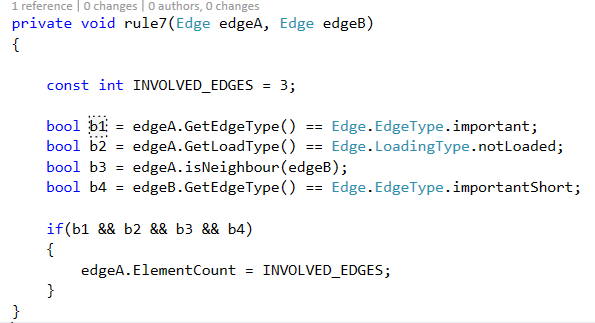
\includegraphics[width=0.9\linewidth]{../Graphics/Rule7Implementation.png}
  \caption{Code implementation of rule 7 provided by dolsak within the RuleManger class}
  \label{fig:sub1}
\end{subfigure}%
\begin{subfigure}{.5\textwidth}
  \centering
  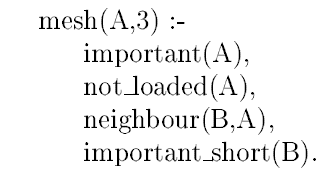
\includegraphics[width=0.7\linewidth]{../Graphics/Rule7Dolsak.png}
  \caption{Rule 7 as stated by dolsak in his papers \cite{appOfILPToFEMeshDesign}}
  \label{fig:sub2}
\end{subfigure}
\label{fig:test}
\end{figure}


\subsection{Mesh Quality Assessment}
Dittmers rules for computing the quality of both individual elements and the entire mesh are built into their own ``MeshQualtyAssessments" and ``ElementQualityMetrics" classes, the latter of which is encapsulated within an element object, like with refinement this allows each element to assess its own quality removing the need for additional utility classes containing static methods. \\

%not sure about the last sentence here
Since each element is initialised with the nodes that comprise it, it is also possible to derive all the geometric characteristics and thus its quality metrics upon its initialisation. This allows the metrics for each node to also be calculated upon its initialisation removing the risk of elements returning null when asked for them.

%Upon evaluation of the project and concluding that effectiveness of the heuristic relied upon overlap of the %heuristically mesh area with areas of high stress

\subsection{Implementation Issues}
Implementation of the design was not without its difficulties, many of which arising as a consequence of unforeseeable complications when implementing the well understood theoretical aspects.


%Think about putting this under evaluation or removing it instead
\subsubsection{Attempts to Automatically Define edges within models}
As discussed under evaluation one of the main issues faced was identifying where the system behaved poorly through weakness in the methods or poor design and implementation as opposed to poor output generated as a consequence of poor input by the operator. In order to avoid this issue it was desirable to try and remove user intervention besides the configuration of the initial model. The obvious way by which to do this was automatic identification of interesting edges within the model. A crucial property which made this approach appear promising is the fact that it is known that edge importance directly correlates with the size of the edge and how much force is applied near it, since both this information exists within the data model it should be possible to identify edges from it and generate them automatically for Dolsaks rules to process.  \\


\noindent
In practice there are multiple complications surrounding this, several of these arise from ambiguity in Dolsaks paper regarding what constitutes a an edge which is for example "long" or "important". As a result edges are only able to be defined to the extent that a user has confidence in their understanding of these concepts. \\ 


Having considered a method using these properties of the mesh several days were then spent attempting to implement it with poor success achieved.
